\documentclass[fontsize=12pt]{article}
\usepackage[utf8]{inputenc}
\usepackage[T1]{fontenc}
\usepackage[german]{babel}
\usepackage{amsmath}
\usepackage{amsthm}
\usepackage{amsfonts}
\usepackage{amssymb}
\usepackage{minted}
\usepackage{tikz}
\usepackage{pgfplots}
\usepackage[top=2cm, bottom=2cm, left=2cm, right=2cm, headheight=1.5cm]{geometry}
\usepackage{fancyhdr}
\usepackage{mdframed}
\usemintedstyle{emacs}

\definecolor{purp}{HTML}{9A72AC}
\definecolor{re}{HTML}{FC6255}
\definecolor{gre}{HTML}{83C167}
\definecolor{blu}{HTML}{58C4DD}
\definecolor{shadecolor}{rgb}{0.85,0.85,0.85}
\definecolor{bg}{rgb}{0.95,0.95,0.95}
\setlength{\parindent}{0em} 

\BeforeBeginEnvironment{minted}{\begin{mdframed}[linewidth =2 ,backgroundcolor=bg , linecolor=black, linewidth=0.5]}
\AfterEndEnvironment{minted}{\end{mdframed}}

\newenvironment{defi}[1]{
    \begin{shaded*}
    \textbf{Definition #1} \\
}{
    \end{shaded*}
}

\newcommand{\bsp}{\textbf{Beispiel}:}
%\newcommand{\task}{\textbf{Aufgabe}:}

\newcommand{\bol}[1]{\textbf{#1}}
\newcommand{\q}[1]{\glqq #1\grqq}
\newcommand{\DODO}[1]{\textbf{\textcolor{red}{DODO:}} #1 \\ \begin{center}\includegraphics[scale=0.2]{../../media/dodo.jpg} \end{center}}

\newenvironment{task}[1]{
    \begin{shaded*}
    \textbf{Aufgabe #1}:
}{
    \end{shaded*}
}



\fancypagestyle{firstpage}{
    \setlength{\headheight}{2.5cm}
    \setlength{\footskip}{0.25cm}
    \pagestyle{fancy}
    \renewcommand{\headrulewidth}{0.4pt}
    \fancyhf{}
    \fancyhead[L]{\LARGE\textbf{Aggregation und Referenzen}}
    \fancyhead[R]{\Large \textbf{Datum:} \hspace{2cm}}
    \fancyfoot[C]{\thepage}
}
\begin{document}
\thispagestyle{firstpage}
\setlength{\headsep}{12pt}
Neben Arrays ist es ein Wesentliches Ziel dieser Jahrgangsstufe, dass in Projekten mehrere Klassen verwendet werden (in kleinerer Form kam dies bereits in der neunten Klasse bei Klassendiagrammen vor!). \\
Damit Objekte verschiedener Klassen einfacher verknüpft werden können, werden sie häufig als Attribute angelegt - bisher waren Attribute hauptsächliche primitive Datentypen wie boolean, int oder double (String war schon die ganze Zeit eine Ausnahme!). \\
Zunächst ein anschaulicheres Beispiel: häufig \q{bestehen} Objekte hauptsächlich aus anderen Objekten (zumindest in der verwendeten Modellierung). Wollen wir beispielsweise ein Stickeralbum modellieren, benötigen wir zwei Klassen, eine für das Album und eine für einen einzelnen Sticker, man kann sagen: das Stickeralbum \textbf{enthält} die Sticker (das entspricht auch der Realität relativ gut!). \\
Im Fachbegriff heißt so eine \q{enthält}-Beziehung \textbf{Aggregation}. Im Objektdiagramm sähe das z.B. so aus: 
\begin{center}
    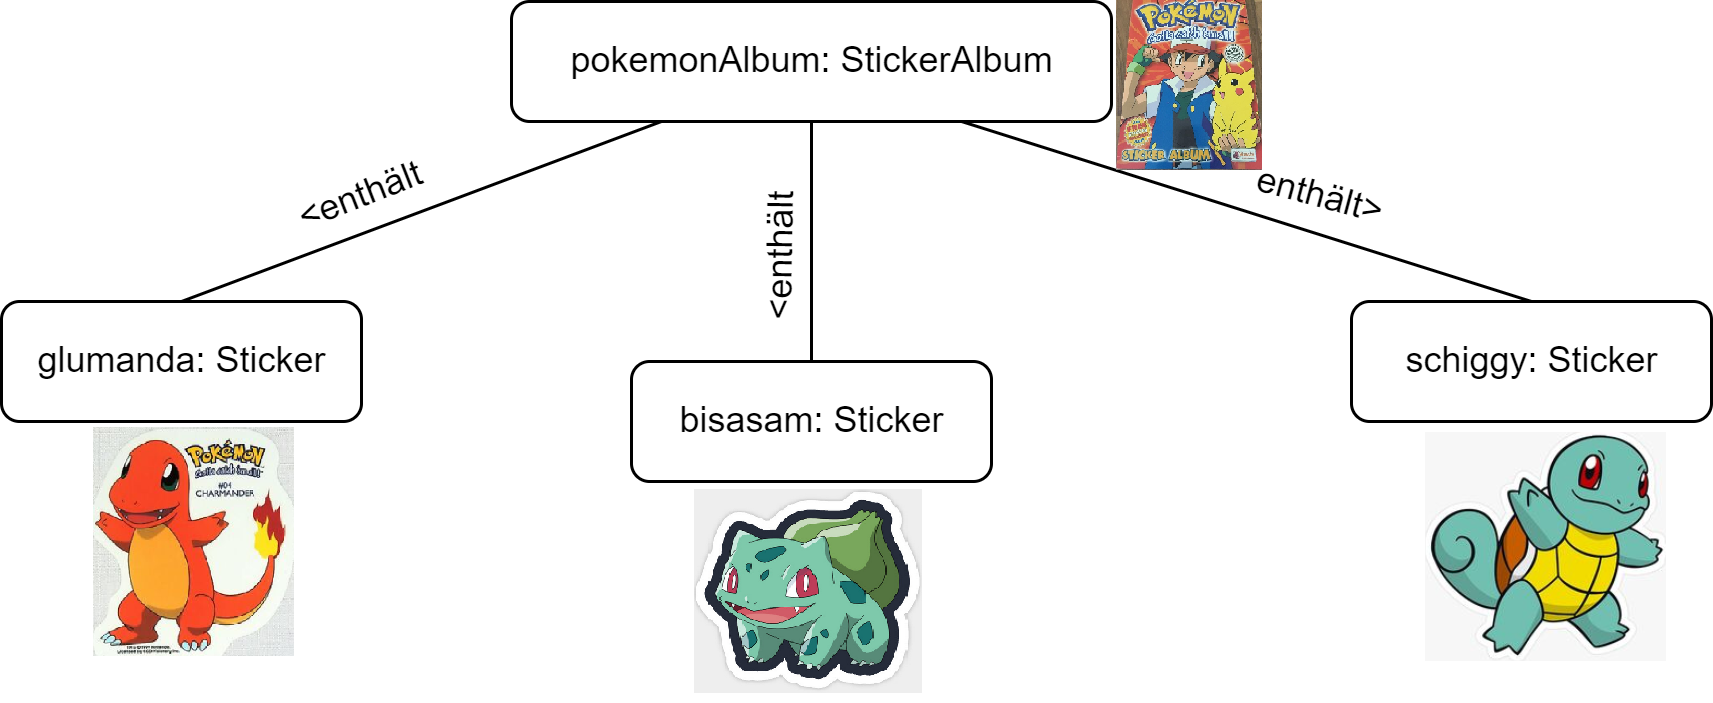
\includegraphics[scale=0.35]{media/obj_diagramm_album.png}
\end{center}
Im Klassendiagramm würde dies mit einem anderen Pfeil markiert werden:
\begin{center}
    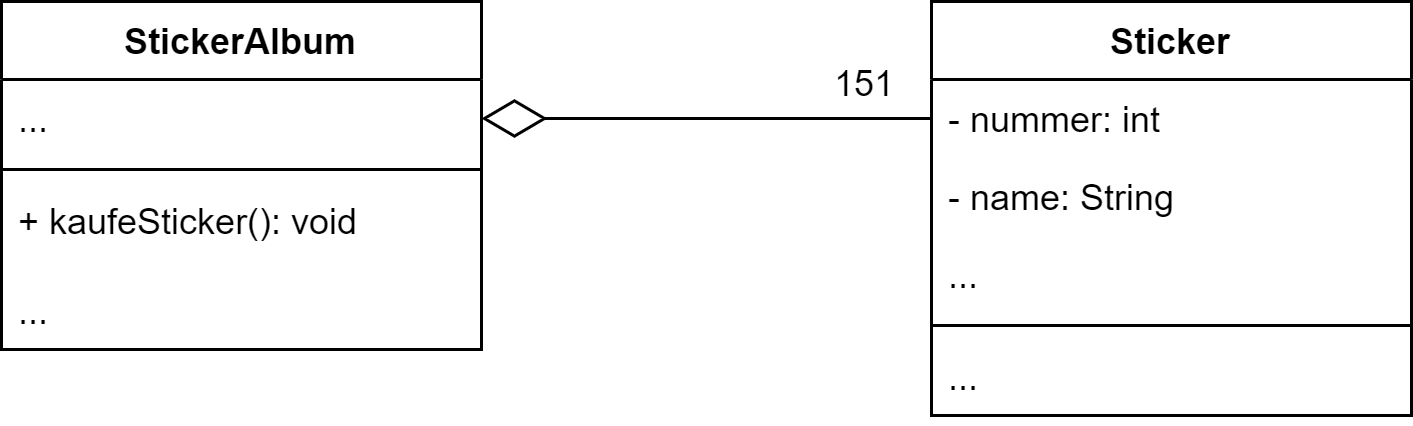
\includegraphics[scale=0.20]{media/class_diagram_album.png}
\end{center}
Ein StickerAlbum besteht also aus 151 Objekten vom Typ Sticker. Die \textbf{Multiplizität} $1$ beim StickerAlbum wird in der Regel weggelassen. Aggregationen werden - wie viele \q{Verbindungen} zwischen Klassen - mit Attributen realisiert. Vereinfachen wir unser Beispiel weiter und nehmen an, dass es nur drei Sticker gibt, dann könnte eine Implementierung so aussehen: 
\begin{minted}{java}
    
\end{minted}
\end{document}